\documentclass[a4papper]{article}

\usepackage{comment, verbatim, listings, graphicx, float, lscape,
  subfigure, wrapfig, placeins, color, amssymb, amsmath}

\lstset{
  language=java,
  breaklines=true,
  basicstyle=\small,
  captionpos=b,
  frame=simple,
  rulesepcolor=\color{black},
  emph={asdf}, emphstyle={\bfseries},
  emph={[2]qwer}, emphstyle={[2]\underbar},
  emph={[3]zxcv}, emphstyle={[3]\underbar}
}
%\lstset{framexleftmargin=5mm, frame=shadowbox, rulesepcolor=\color{blue}} 

\renewcommand{\figurename}{Figura}
\renewcommand{\contentsname}{Indice}
\renewcommand{\lstlistingname}{Codice}

\begin{document}

%\title{}
\title{Relazione del progetto di\\Introduzione all'Audio Digiale:\\Audio Processing Tools}
\author{Federico Mariti}
\maketitle
%\tableofcontents

%% \input{scopo}
%% \input{definizioni}
%% \input{javaAudio}
%% \input{impl_classi}
%% \input{impl_dettaglio}
%% \input{esempio}

Lo scopo del progetto \`e la realizzazione di un programma che
consenta l'elaborazione offline di file audio. Le trasformazioni studiate sono 
\begin{itemize}
\item il cambiamento di volume,
\item la normalizzazione,
\item controllo di tono.
  \end{itemize}
L'applicativo \`e realizzato in modo modulare cos\`i da permettere una
facile estensione dell'insieme di trasformazioni messe a
disposizione. Alcune operazioni di elaborazione audio, ad esempio la
normalizzazione, richiedono la conoscenza di tutto il contenuto
audio. Per facilitare l'implementazione si \`e deciso di copiare in
memoria tutto il contenuto del file audio da elaborare. Il linguaggio
di programmazione scelto \`e Java in quanto fronisce un'interfaccia
audio omogenea rispetto a sistemi operativi diversi e consente di
agire a basso livello sul contenuto audio, con il livello di
astrazione dei dati byte dei campioni audio.

Una operazione di elaborazione audio \`e modellata come un modulo
avente una funzione detta \emph{filter} che assume come parametro un
array di bytes, rappresentate l'audio da elaborare. 
\begin{lstlisting}
  void filter(byte[] data, int off, int len)
\end{lstlisting}
Il modulo \`e inoltre caratterizzato da un formato audio necessario
per interpretare correttamente i bytes audio all'interno della
funzione filter.

L'interfaccia Java \verb+Module+ dichiara i metodi forniti da un
modulo di elaborazione audio:
\begin{lstlisting}
  void filter(byte[] data, int off, int len)
  AudioFormat getAudioFormat()
  void setAudioFormat(AudioFormat af)
\end{lstlisting}
La classe astratta \verb+AbstractModule+ implementa \verb+Module+,
contiene un oggetto di tipo \verb+javax.sound.sampled.AudioFormat+ e
implementa i metodi setter e getter per il fomato audio del modulo, il
metodo \emph{filter} rimane astratto e viene implementato dalle classi
\emph{final} che realizzano lo specifico comportamento di moduli di
elaborazione.

Sono state implementate due diverse interfacce utente: una a riga di
comando e l'altra grafica. Indipendentemente dall'interfaccia utente
le operazioni svolte dal programma sono le seguenti:

\begin{enumerate}
\item apertura di un file audio, selezionato dall'utente,
  \begin {enumerate}
  \item verifica che il formato audio sia supportato,
  \item verifica che la dimensione del file sia completamente
    allocabile in memoria
  \end{enumerate}
\item creazione di un \verb+AudioInputStream+ dal file aperto,
\item mapping in memoria di tutto il contenuto del file,
\item creazione di un modulo di elaborazione audio che implementa la
  trasformazione richiesta dall'utente e esecuzione della sua funzione
  \verb+filter+ sul contenuto del file scritto in memoria,
\item scrittura della trasformazione in un file scelto dall'utente (ha
  lo stesso formato del file di ingresso).
\end{enumerate}

%% \begin{enumerate}
%% \item L'utente fornisce un file audio
%% \item Creazione di un AudioInputStream dal file audio
%% \item Allocazione del contenuto del file in memoria
%% \item L'utente specifica la trasformazione da effettuare
%% \item Viene eseguita l'operazione richiesta
%% \item Il contenuto del file trasformato viene scritto in un file specificato dall'utente
%% \end{enumerate}

\section{Volume}
Nello studio di elaborazioni audio il cambiamento di volume \`e la
prima trasformazione da effettuare in quanto la sua realizzazione \`e
molto semplice. Consiste nell'applicare, tramite moltiplicazione, un
fattore costante a tutti i campioni di ogni canale dell'audio
considerato. Cos\`i facendo si aumenta (se il fattore \`e maggiore di
1) o si riduce l'ampiezza del segnale audio considerato. La buona
realizzazione di tale trasformazione \`e perci\`o delegata alla
corretta interpretazione dei dati audio (dimensione dei campioni
audio, ordinamento dei bytes). L'algoritmo \`e descritto dalla
seguente formula in cui $x[n]$ definisce il segnale audio (di un
canale) di lunghezza n campioni:
%% \begin{lstlisting}
%%   for each sample in data do : sample = sample * volume;
%% \end{lstlisting}
$$ \alpha \in \mathbb{N},\quad \forall i \in \{0, \dots, n-1\} \colon \;
y[i] = \alpha \cdot x[i]$$

L'implementazione Java della funzione \emph{filter} fa uso di
funzionalit\`a di conversione da bytes a interi e viceversa contenute
nella classe \verb+AudioUtils+. L'oggetto \verb+Volume+ che implementa
\verb+Module+ contiene l'oggetto intero \verb+volume+ che rappresenta
il fattore da applicare al segnale audio.
\begin{lstlisting}[caption={La parte rilevante dell'implementazione della funzione filter della classe Volume}]
  for (i=off; i<len; i+=sampleSize) {
    if (2 == sampleSize) 
      next = AudioUtils.byte2int(data[i], data[i+1], isBigEndian);
    else if (3 == sampleSize)
      next = AudioUtils.byte2int(data[i], data[i+1], data[i+2], isBigEndian);
    next = (int)(next * volume);
    byte[] tmp = AudioUtils.int2byte(next, isBigEndian);
    data[i] = tmp[0];
    data[i+1] = tmp[1];
    if (3 == sampleSize) 
       data[i+2] = tmp[2];
  }
\end{lstlisting}
    %% switch(sampleSize) {
    %% case 2:
    %%   next = AudioUtils.byte2int(data[i], data[i+1], isBigEndian);
    %%   break;
    %% case 3: 
    %%   next = AudioUtils.byte2int(data[i], data[i+1], data[i+2], isBigEndian);
    %%   break;
    %% }
%% \begin{lstlisting}
%% ByteArrayInputStream bais = new ByteArrayInputStream(buffer);
%% ByteArrayOutputStream baos = new ByteArrayOutputStream();
%% DataInputStream dis = new DataInputStream(bais);
%% DataOutputStream dos = new DataOutputStream(baos);
%% try {
%%   while (true) { 
%%     next = Short.reverseBytes(dis.readShort());
%%     next = (int)(next * volume);
%%     dos.writeShort(Short.reverseBytes(next));
%%   }
%% } catch(EOFException e) { ; }
%% \end{lstlisting}

\section{Normalizzazione}
La normalizzazione di una informazione audio consiste nell'aumentare
l'ampiezza del segnale audio in modo costante per tutta la durata del
segnale cos\`i da renderla massima e non introdurre distorsione. Si
tratta di un caso particolare di aumento di volume, il fattore di
incremento \`e scelto analizzando tutto il segnale audio e portando il
picco pi\`u alto al massimo valore rappresentabile dalla dimensione
del campione. \`E possibile sceglire di normalizzare anche ad un
valore inferiore a quello massimo.

L'implementazione \`e simile a quella del modulo \emph{volume}, ne
differisce per una prima scansione di tutto il contenuto audio,
ricercando il valore massimo in valore assoluto dei campioni, senza
fare distinzione tra i canali. Quindi il fattore di \emph{gain} viene
calcolato come:
\begin{lstlisting}
int upperBound = 1 << af.getSampleSizeInBits();
if (af.getEncoding() == AudioFormat.Encoding.PCM_SIGNED)
   upperBound = upperBound / 2;
upperBound = upperBound - 1;
gain = upperBound * (targetLevel/100F) / maxPeak;
\end{lstlisting}
Dove \verb+af+ \`e l'oggetto che rappresenta il formato audio del
segnale, \verb+targetLevel+ \`e il valore di normalizzazione scelto
dall'utente e \verb+maxPeak+ \`e il valore del picco pi\`u alto
trovato nel segnale audio. Successivamente viene eseguito lo stesso
algoritmo di \emph{volume} usando \verb+gain+ come valore di volume.

\section{Controllo di tono}
Per controllo di tono si intende una alterazione dello spettro di
tutto il segnale audio considerato, tale elaborazione \`e una
trasformazione lineare e invariante nel tempo. Il modulo implementato
realizza un filtro digitale della famiglia FIR (Finite Inpulse
Response). Filtri di questo tipo si basano sull'operazione matematica
di convoluzione di due segnali, il filtro viene modellato come un
sistema lineare e invariante nel tempo, e perci\`o descritto
completamente dalla sua risposta alla funzione impulso. Il
comportamento del filtro \`e una combinazione lineare di un gruppo
consecutivo di campioni del segnale considerato. Sia $x[n]$ il segnale
audio considerato composto da $n$ campioni, si indica con $x[i]$ la
componente i-esima del segnale x. La risposta impulsiva del filtro \`e
un segnale di $k$ componenti, in genere $n >> k$, la componente
i-esima del filtro, anche detta coefficiente i-esimo del filtro, \`e
indicata con $c_i$. Il comportamento del filtro \`e specificato dalla
seguente relazione, con $y[n]$ il segnale risultato:
%% Per implementare il controllo di tono viene usata la tecnica del
%% Finite Impulse Response (FIR), l'elaborazione avviene sui dati del
%% dominio del tempo, la modellazione del filtro
%% $$ x[n] \in \mathbb{Z}^n, \quad c \in \mathbb{Z}^k, \quad n >> k$$
%% $$ \forall i \in \{0, \dots, n-1\} \colon \; y_i = \sum_{j=0}^{k} c_j \cdot x_{i-j} $$
$$ \forall i \in \{0, \dots, n-1\} \colon \; y[i] = \sum_{j=0}^{k-1} c_j \cdot x[i-j] $$
Ovvero la componente i-esima del segnale risultato \`e una
combinazione lineare (definita dai coefficenti del filtro) dei k
componenti di $x$ precedenti a $x[i]$. Il calcolo delle componenti di
$y$ pu\`o essere descritto con il seguente algoritmo:\\

$ \forall i \in \{0, \dots, n-1\} :$

$ \qquad y[i] := 0 $

$ \qquad\forall j \in \{0, \dots, k-1\} :$

$ \qquad \qquad $ \textbf{if} $ i-j > 0 \; \land \; i-j < n \; $ \textbf{then} $ \; y[i] := y[i] + c_j \cdot x[i-j] $
\\

\begin{figure}[!b]
  \centering
  \resizebox{\columnwidth}{!}{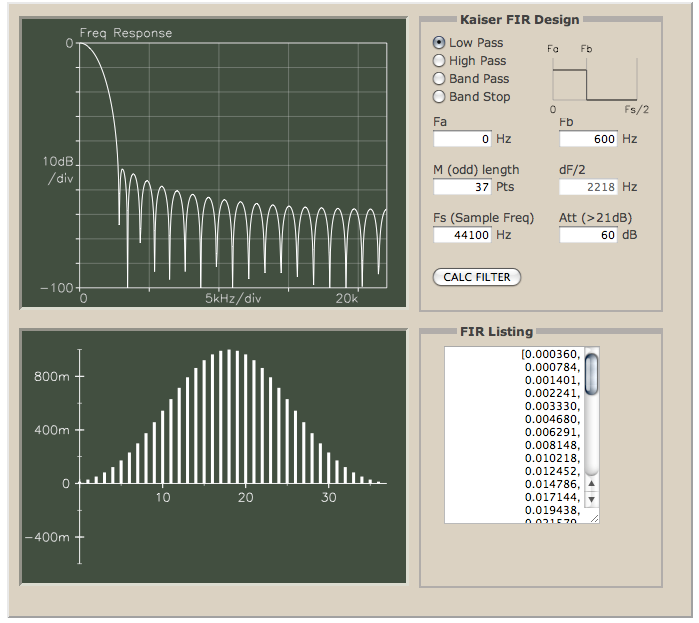
\includegraphics{digital_filter_design.png}}
  \caption{Schermata dell'applicativo la definizione del filtro e il
    calcolo dei relativi coefficenti}
  \label{}
\end{figure}

La definizione del filtro e quindi dei suoi coefficienti viene
effettuata con l'ausilio di un'applicazione esterna, ad esempio\\
\verb+http://arc.id.au/FilterDesign.html+. Il programma richiede che
l'utente specifichi un file testuale contenente i coefficenti del
filtro, analizza il file e salva i coefficienti nell'oggetto che
implementa il modulo.

Di seguito viene fornita l'implemetazione Java della funzione
\emph{filter} del modulo che realizza il comportamento di un FIR. Tale
implementaizone segue l'algor\-itmo presentato
precedentemente. All'interno di tale funzione viene usato un array di
interi come array circolare per memorizzare i $k$ campioni audio di
$x$ necessari al calcolo del campione attuale del risultato. Al
calcolo di una generica componente $y[i]$, il valore di $x[i]$ viene
decodificato dallo stream di bytes del segnale audio e scritto nella
posizione corrente del buffer circolare, rimpiazzando cos\`i il valore
pi\`u vecchio presente nel buffer.

%% \begin{align}
%% \forall i& \in \{0, \dots, n-1\} :\\
%% &y[i] := 0\\
%% &&\forall j& \in \{0, \dots, k-1\} :\\
%% &&&i
%% \end{align}

\begin{lstlisting}
  //define: tail is the index of the next buffer element to
  //        write, that is, tail is the index of the oldest
  //        element in buffer
  int tail = 0;
  int[] buffer = new int[coef.length];
  for (int i=off; i<len; i+=sampleSize) {
    // y[i] = 0
    result = 0;
    // x[i]
    if (2 == sampleSize) 
      buffer[tail] = AudioUtils.byte2int(data[i], data[i+1], isBigEndian);
    else if (3 == sampleSize)
      buffer[tail] = AudioUtils.byte2int(data[i], data[i+1], data[i+2], isBigEndian);
    for (int j=0; j<coef.length; j++) {
      if (i-j > 0 && i-j < len) {
	// y[i] = y[i] + c[j] * x[i-j]
	int index;
	if (tail-j < 0) index = buffer.length + tail - j;
	else            index = tail-j;
	result += coef[j] * buffer[index];
      }
    }
    byte[] tmp = AudioUtils.int2bytes((int)result, isBigEndian);
    data[i] = tmp[0];
    data[i+1] = tmp[1];
    tail = (tail+1) % coef.length;
  }
\end{lstlisting}
\FloatBarrier

\section{Esempi di uso}
\subsection{Command line interface}
La stampa di aiuto del programma:
\begin{verbatim}
$ java mariti.audio.iad.CommandLineInterface -h
usage: -f inputFile -m moduleName [-a argName=value ...] -o outputFile
  -a,--argument
  -f,--file <fileName>        The input audio file
  -h,--help                   Shows the help content
  -m,--module <moduleName>    The audio processig module name
  -o,--output-file <fileName> The output audio file
Modules arguments:
  volume: -a volume=<integer>
  peakNormalization: -a peak=<integer>
  lowPass: nothing
  fir: -a file=<fileName>
  fir: -a coefficients=<float,float,...>
\end{verbatim}
Esempio di uso del programma per la modifica di tono:
\begin{verbatim}
$ java mariti.audio.iad.CommandLineInterface -f "500 miles high.wav" \
  - o out.wav -m fir -a file=coef_lowPass_44100.txt
\end{verbatim}
L'invocazione del programma richiede il file audio su cui effettuare
l'elaborazione, il file audio di uscita contenente il risulato
dell'elaborazione, e il modulo di elaborazione con i relativi
argomenti. Una singola invocazione del programma produce una singola
trasformazione.

\subsection{Graphical user interface}
Vengono presentate le stampe del programma con i diversi moduli di
elaborazione. La finestra dell'applicazione \`e composta da 4 sezioni
disposte lungo l'asse verticale: 
\begin{itemize}
\item i controlli del pannello superiore consentono di definire il
  file audio su cui effettuare l'elaborazione,
\item il pannello centrale \`e uno schedario che consente di scegliere
  quale modulo di elaborazione usare, all'interno dello schedario
  vengono presentati i componenti che definiscono i valori degli
  argomenti del modulo correntemente selezionato.
\item i controlli del terzo pannello consentono di definire il
  file audio su cui scrivere l'elaborazione,
\item il pannello pi\`u basso presenta il pulsante di scrittura, la
  pressione di tale pulsante aziona l'esecuzione dell'operazione
  specificata dai controlli nei pannelli superiori.
\end{itemize}
A differenza del programma a riga di comando \`e perci\`o possibile
effettuare pi\`u elaborazioni all'interno di una singola esecuzione del
programma.
\begin{figure}[!h]
  \centering
  \resizebox{\columnwidth}{!}{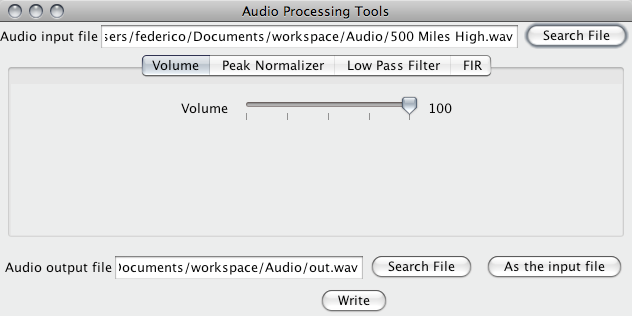
\includegraphics{window_volume.png}}
  \caption{Schermata del modulo volume}
  \label{}
\end{figure}

\begin{figure}[!h]
  \centering
  \resizebox{\columnwidth}{!}{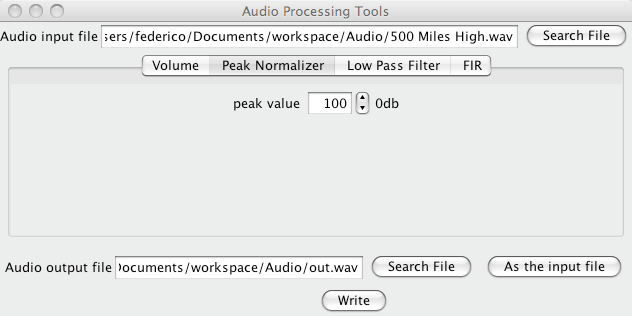
\includegraphics{window_peakNormalizer.png}}
  \caption{Schermata del modulo normalizzatore}
  \label{}
\end{figure}

\begin{figure}[!h]
  \centering
  \resizebox{\columnwidth}{!}{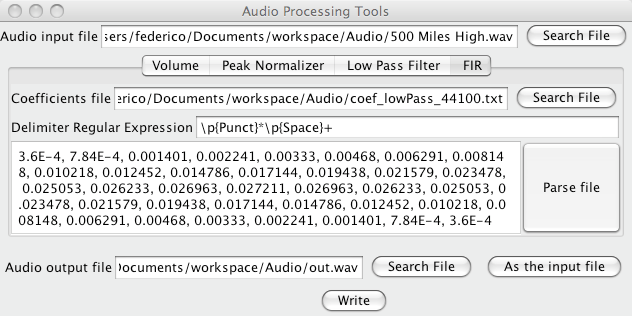
\includegraphics{window_fir.png}}
  \caption{Schermata del modulo FIR}
  \label{}
\end{figure}
\FloatBarrier
Nella scheda del modulo FIR viene chiesta la definizione di un file
testuale contenente i coefficenti del filtro da applicare, tale file
pu\`o avere un formato arbitrario ed \`e specificato da una espressione
regolare. Una volta scelto il file dei coefficenti, il suo contenuto
viene mostrato in una regione di testo modificabile con formato di
delimitazione delle componenti ``virgola e spazio''.

\end{document}
